\documentclass[10pt, a4paper]{article}
\usepackage{float}
\usepackage{geometry}
\usepackage{listings}
\usepackage{hyperref}
\usepackage{graphicx}
\usepackage{ragged2e}
\usepackage{color}
\usepackage{xepersian}
\usepackage{subfiles}
\newgeometry{left=2.4cm, right=2.4cm, bottom=2.4cm, top=2.4cm}
\settextfont[Scale=1]{XB Roya}
\usepackage{multirow}
\renewcommand{\baselinestretch}{1.5}
\definecolor{dkgreen}{rgb}{0,0.6,0}
\definecolor{gray}{rgb}{0.5,0.5,0.5}
\definecolor{mauve}{rgb}{0.58,0,0.82}
\definecolor{commentColor}{rgb}{0.6,0.6,0.60}
% Code style configuration
\lstset{frame=tb,
  language=python,
  aboveskip=1mm,
  lineskip=0.9mm,
  belowskip=1mm,
  showstringspaces=false,
  showspaces=false,
  columns=flexible,
  basicstyle={\small\ttfamily},
  numbers=none,
  keywordstyle=\color{mauve},
  commentstyle=\color{commentColor},
  stringstyle=\color{dkgreen},
  numberstyle=\small\color{black},
  numbers=left,
  stepnumber=1,
  breaklines=true,
  breakatwhitespace=true,
  tabsize=3
}

\title{گزارش بررسی پیکربندی نامناسب سرویس‌های NoSQL در مقیاس پروژه‌های در سطح
جهان به تفکیک ابزار‌ها و موتور‌های NoSQL}
\author{\href{mailto:a.soltani@iau-tnb.ac.ir}{علیرضا سلطانی نشان} \small{استاد
راهنما: آقای دکتر شجاعی مهر}}

\begin{document}

\maketitle

دانشگاه آزاد اسلامی، واحد تهران-شمال، دانشکده فنی مهندسی کامپیوتر، گرایش مهندسی
نرم‌افزار، مقطع کارشناسی ارشد

\section{مجوز}

به فایل license همراه این برگه توجه کنید. این برگه تحت مجوز GPLv3 منتشر شده است
که اجازه نشر و استفاده (کد و خروجی/pdf) را رایگان می‌دهد.

\section{تعریف مسئله}

ذخیره‌سازی اطلاعات از مهم‌ترین نیاز‌های تحلیل کنندگان داده است. امروزه با توجه
به پیشرفت صنعت IoT و یادگیری ماشین، تولید داده‌ها بسیار افزایش یافته است به
گونه‌ای که بتوان این داده‌ها را به سریع‌ترین روش ممکن در محلی مناسب ذخیره‌سازی و
نگهداری کرد.  افراد برای ذخیره‌سازی این داده‌ها نیاز به نصب و راه‌اندازی یک
سیستم DBM دارند که از طریق یک واسط با زبانی مناسب بتوانند به آن متصل شده و
داده‌های دریافتی را بعد از تجزیه و تحلیل آنها در این محل ذخیره‌سازی و مدیریت
کنند. امروزه محققان ترجیح می‌دهند به دلیل مقیاس پذیری بیشتر، سیستم‌های توزیع شده
و قابلیت پایداری بالا از دیتابیس‌های رابطه‌ای به سمت دیتابیس‌های NoSQL مهاجرت
کنند.  این نوع دیتابیس‌ها امروزه توسط تمام اپلیکیشن‌های جدید پشتیبانی می‌شوند و
برای استفاده آسان طراحی شده‌اند. حتی می‌توان متذکر شد که تعداد زیادی از
سرویس‌های ذخیره‌سازی ابری امروزه‌ از سرویس‌های دیتابیسی NoSQL پشتیبانی گسترده‌ای
دارند. این ارائه دهندگان اغلب شرکت‌های معروفی مانند \lr{Amazon DynamoDB}
\lr{Google Cloud Database} \lr{MS Azure CosmosDB} می‌باشند. همچنین بیشتر این
موتور‌های دیتابیسی به صورت متن‌باز هستند و توسعه دهندگان زیادی از سرتاسر جهان
روی آنها مشغول توسعه هستند.

در سال‌های اخیر، با پدید آمدن و رشد سریع سرویس‌های دیتابیسی NoSQL بین عموم
توسعه‌دهندگان استفاده از این نوع سرویس‌ها افزایش یافته است. دلیل اصلی این
محبوبیت نصب و راه‌اندازی و استقرار آسان آنها در هر محلی است. همچنین قابل اعتماد
هستند، روش‌ها و مکانیزم‌های زیادی برای تهیه نسخه‌های پشتیبان‌گیر به صورت منظم از
داده‌ها را ارائه می‌دهند. دلیل اصلی آسان بود این سیستم آن است که در هنگام
راه‌اندازی آنها زمان زیادی را صرف نمی‌کنید، زیرا بعد از نصب اولیه و طی کردن
فرایند نصب با زدن روی دکمه "بعدی" دیتابیس شما آمادست و می‌توانید از آن در برنامه
خود استفاده کنید. بعد از این فرایند هیچ عملیاتی بر روی تعریف دسترسی‌ها، مدیریت
کاربران در استفاده از دیتابیس مانند اختصاص سطح دسترسی، توسط راه‌انداز سیستم DBM
صورت نمی‌گیرد. نتیجه این موارد پیکربندی غیر اصولی و اشتباه
\footnote{Misconfigured} سیستم ذخیره‌سازی داده می‌شود که در نتیجه افشای اطلاعات
حساس \footnote{\lr{Data Leakage}} را به دنبال خواهد داشت.

سوالی که ممکن است در اینجا مطرح شود آن است که چه زمانی پیکربندی نادرست موجب
افشای اطلاعات می‌شود؟

در ابتدا بعد از راه‌اندازی این نوع دیتابیس‌ها اولین هدف استفاده از آنها در محیط
لوکال در یک شبکه است. اما افشای اطلاعات و پیکربندی اشتباه زمانی رخ می‌دهد که این
دیتابیس‌ها در شبکه اینترنت مورد دسترسی قرار گیرند.

محققان با توجه به موارد گفته شده بالا توانسته‌اند یک ابزار خودکار جهت آنالیز و
جست و جوی سیستم‌های دیتابیسی NoSQL را توسعه دهند که به وسیله آن می‌توانند
پیکربندی نامناسب این سیستم‌های مستقر شده را متوجه شده، موارد آسیب‌پذیری را گزارش
و سپس به صاحبان این دیتابیس‌ها هشداری در جهت در خطر بودن اطلاعاتشان ارسال کنند.

در این گزارش به طور خلاصه تمام موارد انجام شده را در پنج عنوان توضیح می‌دهیم. در
ابتدا در مورد چالش‌ها و نحوه تحقیق روی این آسیب پذیری‌ها و عدم وجود پیکربندی
مناسب می‌پردازیم. در بخش مدل پیشنهادی بیشتر ماهیت ابزار توسعه داده شده را مطرح
می‌کنیم و سپس نتایج اجرای این ابزار را نمایش می‌دهیم و در نهایت به نوآوری و
کار‌های آینده می‌پردازیم.

\section{چالش‌ها}

ابزاری توسعه داده شده است که در یک رنج گسترده‌ای از آدرس‌های IP می‌تواند اینگونه
دیتابیس‌ها را اسکن کند و افشای سرویس آنها را تشخیص دهد. این تشخیص به شکل ایمن
بدون هیچ نگهداری داده‌ها و یا افشای اطلاعات حساس آنها صورت می‌گیرد. بررسی ضعف
پیکربندی‌های صورت گرفته بر روی ۶۷ میلیون ۷۲۶ هزار و ۶۴۱ آدرس IP بوده است که بین
بازه زمانی اکتبر ۲۰۱۹ و مارچ ۲۰۲۰ تکمیل شده است. نکته جالب از آنجایی شروع می‌شود
که این سرویس‌ها نه تنها به صورت شخصی راه‌اندازی شده‌اند بلکه تعداد ۱۲ هزار و ۲۷۶
نمونه از آنها در ارائه دهندگان سرویس‌های ابری معروف یافت شده است.  با توجه به
این موضوع در این تحقیق ۷۴۲ مورد آسیب پذیری پیدا شده است که به صورت مستقیم وب
سایت این کاربران به دلیل ضعف در پیکربندی به دیتابیس‌های آنها ارجاع دارد این بدان
معناست با وجود تنظیمات و پیکربندی پیش فرض و بدون هیچ گونه استراتژی امنیتی، هر
کاربر ناشناس دیگری می‌تواند وارد این دیتابیس‌ها شده و آنها را با نظر و سلیقه
خودش تغییر و حتی تخریب به قصد اخاذی کند.

\subsection{بررسی نمونه‌ها در پیکربندی ضعیف راه‌اندازی}

\begin{enumerate}
    \item در مارچ ۲۰۲۰، ۷ ترابایت از داده‌های سایت بزرگسالان به صورت صریح از یک
    نمونه دیتابیس \lr{Elastic Search} با اطلاعاتی از قبیل، نام کاربران، جنسیت و
    گرایش‌ها، لاگ‌های مربوط به پرداخت‌هایشان، ایمیل، با ۱۰۸۸ میلیارد رکورد مورد
    افشا قرار گرفت.
    \item در نوامبر سال ۲۰۱۹ یک محقق توانست یک نمونه با پورت باز با بیشتر از ۱/۲
    میلیارد رکورد از یک دیتابیس را پیدا کند که شامل اطلاعات حساس کاربران از قبیل
    آدرس ایمیل آنها بود.
    \item در ژانویه سال ۲۰۱۷، در یک حمله بیشتر از ۶۰۰ نمونه از دیتابیس
    \lr{Elastic search} حذف شدند و برای بازیابی آنها از صاحبانشان اخاذی کردند
    \cite{mongoransacked}.
    \item براساس گزارشی در سال ۲۰۱۸ بیشتر از ده ها هزار نمونه از دیتابیس‌های
    Redis در دسترس کاربران مخرب، آسیب‌پذیر شناخته شدند که به دلیل دسترسی عموم
    افراد تعداد ۷۵۰۰ سرور یافت شد که در معرض خطر یک بدافزار به نام Botnet بودند
    که هدف اصلی آنها دزدیدن ارز‌های دیجیتال \footnote{Cryptocurrencies} آن
    پلتفرم ارائه دهنده بود.
\end{enumerate}

براساس موارد مطرح شده در بند‌های گفته شده بالا، اولین بررسی از ضعف پیکربندی
دیتابیس‌های NoSQL انجام شده است به گونه‌ای که می‌توان از آن برای تشخیص و تعیین
معیاری برای بررسی پیکربندی درست در این دیتابیس‌ها از آن استفاده کرد. محققان یک
فریمورکی توسعه داده‌اند که به صورت کاملا خودکار می‌تواند سرویس‌های معرض دید عموم
را تشخیص و عملیات بررسی امنیتی روی آنها انجام دهد بدون ذخیره‌سازی داده‌های
کاربران یا باز کردن داده‌های دیتابیس پلتفرم‌ها و دریافت اطلاعات حساس آنها.

\subsection{فرایند کلی عملکرد فریمورک \cite{ferrari2020nosql}} 

این فریمورک در ابتدا لیستی از آدرس‌های IP که توسط بیشتر ارائه دهندگان سرویس‌های
ابری استفاده می‌شود را اسکن کرده و به دنبال ارتباطی باز بر روی پورت پیش فرض
دیتابیس NoSQL می‌گردد که بتواند به آن به صورت مستقیم متصل شود. (در شکل ۱،
می‌توانید عملکرد فریمورک را در تصویر مشاهده کنید.) سپس می‌تواند به یک نمونه از
دیتابیس دسترسی داشته و عملیات بررسی امنیتی خود را شروع کند.  به طور کلی این
فریمورک به بررسی سطح دسترسی دیتابیس (همان دسترسی‌های خواندن و نوشتن روی یک سیستم
مدیریت دیتابیس) متا دیتا از قبیل نسخه مورد استفاده از سرویس ،NoSQL کاربران مجاز
دسترسی به دیتابیس، سطوح دسترسی تعریف شده و جداول مرتبط به این دیتابیس‌ها،
می‌پردازد. 

\begin{figure}[H]
    \centering
    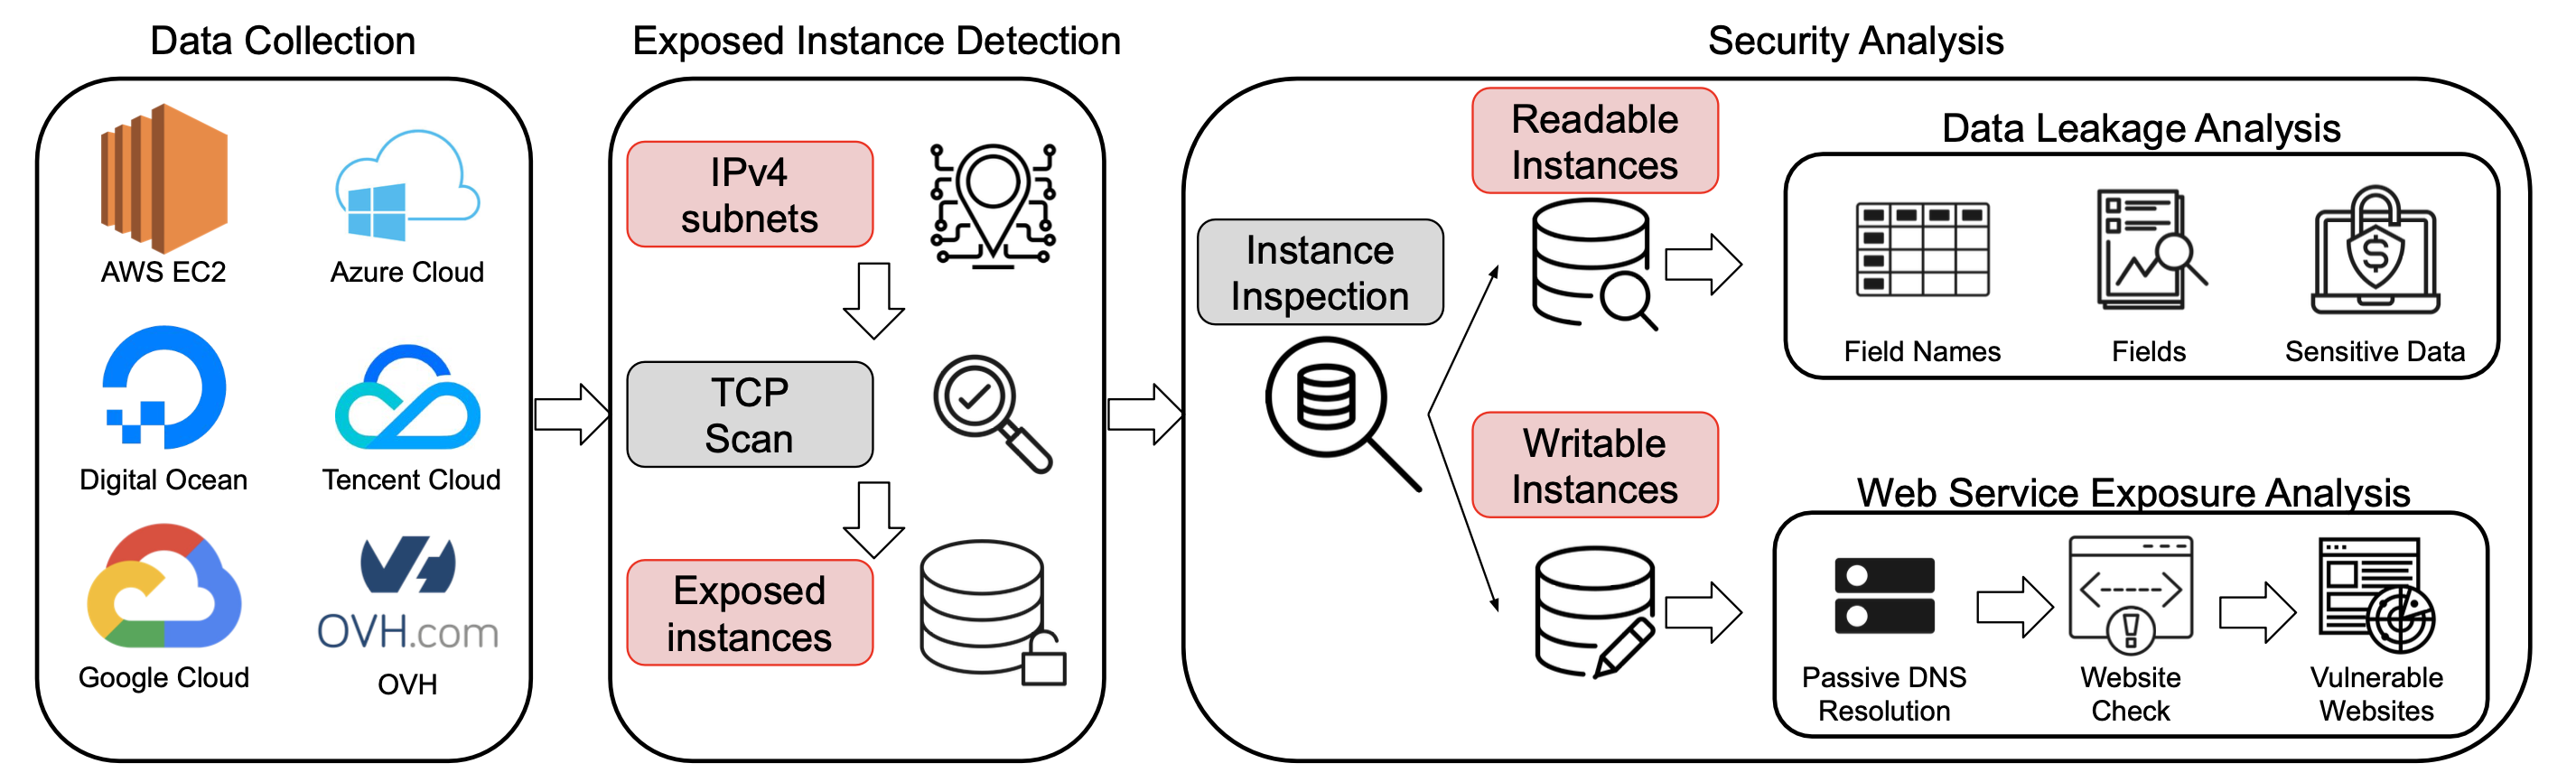
\includegraphics[width=1\textwidth]{res/fig1.png}
    \caption{بررسی عملکرد ابزار توسعه داده شده}
    \label{fig: diagram}
\end{figure}

\subsubsection{تشخیص عمل خواندن از دیتابیس‌های فاش شده}

اگر این ابزار تشخیص دهد که دسترسی خواندن را از این دیتابیس‌ها دارد تضمین افشای
اطلاعات این سیستم‌ها را به طور قطعی می‌دهد که می‌تواند خطری برای محتوای داخل
دیتابیس باشد. ابزاری که توسعه داده شده است کاملا ایمن می‌باشد چرا که اصلا وارد
محتوای این دیتابیس‌ها و داده‌های آنها نشده و تنها از توابعی مانند تابع Count
برای شمارش رکورد‌هایی که مربوط به فیلد‌هایی مانند نام کاربران، شماره تلفن یا
آدرس ایمیل آنها می‌شود، استفاده می‌کند. اغلب داده‌های جمع‌آوری شده از این
دیتابیس‌ها به صورت نمایش تعداد رکورد‌های آنها مربوط به فیلدی مشخص است که در
جداول صفحات بعدی آنها را مشاهده خواهید کرد.

\subsubsection{تشخیص عمل نوشتن از دیتابیس‌های فاش شده}

زمانی که این ابزار بتواند به این دیتابیس‌ها متصل شود و بعد از آن قادر به ساخت یک
workspace یا یک رکوردی از داده‌ NoSQL یعنی همان Document باشد، تشخیص می‌دهد که
مجوز نوشتن را در این سیستم دارد به همین خاطر یک پیام جدی را برای صاحبان دیتابیس
می‌نویسد تا در جریان ضعف پیکربندی و ایمن نبودن ارتباطات آنها و باز بودن
دسترسی‌ها، قرار بگیرند. با این کار محققان از افشا و آسیب به نمونه از دیتابیس
جلوگیری می‌کنند. داشتن دسترسی نوشتن یکی از خطرناک‌ترین دسترسی‌های این دیتابیس‌ها
می‌باشد به طوری که این ابزار علاوه عملیات گفته شده بالا یک استراتژی دیگری را در
پیش می‌گیرد و آن این است که به جست و جوی DNS های آن به صورت غیر فعال می‌پردازد
تا متوجه آن شود که آیا روی این IP که دیتابیس مستقر شده است، منابع دیگری مانند
برنامه‌های وب و وبسایت‌ها و دیگر سرویس‌ها مستقر شده‌اند یا خیر؟ چرا که اگر منابع
وب را از این طریق پیدا کند به این معنی است که این سرور‌ها پتانسیل حمله
آسیب‌زننده‌ای که باعث دستکاری داده‌ها می‌شود را دارند. در تمام وضعیت گفته شده
بالا با ارائه دهندگان سرویس‌های ابری ارتباط برقرار شده و به آنها در مورد
آسیب‌پذیری‌های یافت شده گزارشی به عمل آمده است.

۶۷ میلیون آدرس IP اسکن شده در ارائه دهندگان سرویس‌های ابری مختلف بین اکتبر سال
۲۰۱۹ تا مارچ ۲۰۲۰، تعداد ۱۲,۲۷۶ سرویس دیتابیسی با دسترسی‌های مختلف یافت شدند که
۸۷٪ آنها با دسترسی آزاد خواندن و نوشتن و ۸/۶٪ آنها تنها قابلیت خواندن اطلاعات را
داشتند. بین این بررسی محققان مواردی از قابل دسترس بودن اطلاعات فقط خواندنی این
دیتابیس‌ها پیدا کردند که ۷۴۲ نمونه پتناسیل افشای اطلاعات حساس کاربران مانند آدرس
ایمیل، نام‌ها، گذرواژه‌ها و تمام منابعی که می‌تواند در اپلیکیشن‌های وب آنها
استفاده شود، را داشتند. علاوه‌بر این ما دیتابیس‌های مختلفی را پیدا کردیم که
توانایی افشای فایل‌های مهم و حساس مانند فایل‌های سرتیفیکیت سایت‌ها و لاگ‌های
مربوط به آنها را داشتند. بین تمام سیستم‌های DBM سرویس MongoDB بیشترین مقدار ضعف
پیکربندی را داشت به گونه‌ای که ۴،۸۵۹ نمونه از آن یافت شد و این سهم برای دیتابیس‌
Elasticsearch به مقدار ۴،۷۲۵ نمونه بود.

\subsubsection{مرور سناریو‌های تهدیدآمیز}

\subsubsection*{افشای اطلاعات (سطح دسترسی خواندن)}

زمانی که منابع دیتابیسی به صورت غیر عامدانه‌ای مورد دسترسی عموم قرار می‌گیرد که
موجب مسائل شکسته شدن حریم خصوصی کاربران و افشای اطلاعات حساس و عدم محرمانگی
می‌شود.

\subsubsection*{آلوده شدن منابع وب (سطح دسترسی نوشتن)}

زمانی که دسترسی نوشتن روی یک میزبان فعال باشد به معنای آن است که تمام محتوای آن
میزبان را می‌توان دستکاری کرد. اغلب وب سایت‌ها به این ترتیب تغییر چهره روی آنها
اعمال می‌شود که مربوط به عملیات دستکاری Deface کردن این پایگاه‌های اطلاعاتی است.
همچنین این عمل باعث تاثیر روی محتوای این وب‌سایت‌ها خواهد شد چرا که می‌توانند
وارد دیتابیس شده و اطلاعات مروبطه را دستکاری کنند و به نفع خودشان ویرایشی انجام
دهند. همچنین آسیب‌پذیری‌های دیگر نیز می‌تواند رخ دهد. برای مثال بعد از دسترسی
نوشتن روی این میزبان‌ها می‌توانند از طریق وب‌سایت یک فایل مخرب و آلوده را قرار
داده و کاربران آن را به عنوان فایل مورد نظر بارگیری کرده و باعث آلوده شدن دستگاه
کاربران نهایی شود.

\subsubsection{اخاذی در ازای اطلاعات}

مهاجمان می‌توانند با داشتن دسترسی نوشتن روی این دیتابیس‌ها حمله‌ای انجام دهند که
موجب اخاذی از صاحبان اطلاعات شود. معمولا استراتژی مهاجمان در این خصوص از بین
بردن اطلاعات یا رمزنگاری‌ آنها می‌باشد که در ازای اخاذی از صاحبان دیتابیس یا
داده می‌توانند داده‌ها را به آنها برگردانند یا آنها کلید رمزنگاری آن داده‌ها را
تحویل دهند.

محققان چهار تا از محبوب‌‌ترین دیتابیس‌های NoSQL را مورد بررسی قرار دادند تا نشان
دهند که تحقیقات آنها کافی بوده و تقریبا مهم‌ترین سرویس‌های NoSQL را پوشش داده
است. محققان تحقیقاتی را نسبت به محبوب‌ترین سیستم‌های دیتابیسی براساس وب سایت
\href{https://db-engines.com/en/ranking}{db-engines.com} به عمل آوردند. مهم‌ترین
سوال آن است که چگونه یک سیستم به عنوان محبوب‌ترین سیستم دیتابیسی انتخاب می‌شود؟

انتخاب این دیتابیس‌ها براساس درصد استفاده آنها در وبسایت‌ها، بحث و گفت و گو‌های
گروه‌های فنی، پیشنهادات شغلی در رابطه با متخصص مربوط به این دیتابیس‌ها و
ارتباطشان در شبکه‌های اجتماعی می‌باشد. براساس جدول ۱، رنک دیتابیس‌های مختلف
براساس سایت db-engines آمده است. لازم به ذکر است که این جدول نسبت به جدول داخل
مقاله به روز شده که طی ۳ سال گذشته دیتابیس‌های Redis و Elasticsearch به ترتیب
مقال ۶ و ۷ را بدست آوردند. در حالی که بین سال ۲۰۱۹ تا ۲۰۲۰ مقام Redis و
Elasticsearch به ترتیب ۷ و ۸ بود \cite{dbengines}.

\subsubsection{اهداف تحقیق}

اهداف این تحقیقات به شرح زیر می‌باشد:

 \begin{enumerate}
    \item نتیجه عدم تدابیر امنیتی
    \item بررسی تاثیر ضعف پیکربندی
    \item افزایش آگاهی برای جلوگیری از فاش شدن و دستکاری اطلاعات
 \end{enumerate}

همچنین در بخش‌های بعدی در مورد آگاهی از نگرانی‌های اخلاقی مطرح شده است که در آن
به جمع‌آوری داده‌‌های نتیجه این آزمایشات صرفا برای بررسی محاسبات محققان نسبت به
آسیب‌پذیری داده‌ها در آینده است.

\begin{LTR}
    \begin{table}[h]
        \centering
        \begin{RTL}
            \caption{رنکینگ موتور‌های دیتابیس: ۱۰ دیتابیس محبوب از نظر سایت db-engines}
        \end{RTL}
        \scalebox{0.7}{
            \begin{tabular}{c|c|c|c|c|c|c|c}
            \multicolumn{3}{c|}{\textbf{رنک}} & {\textbf{دیتابیس‌}} & {\textbf{مدل}} & \multicolumn{3}{c}{\textbf{امتیاز}} \\
            \hline
                \textbf{نوامبر ۲۰۲۳} & \textbf{اکتبر ۲۰۲۳} & \textbf{نوامبر ۲۰۲۲} & & & \textbf{نوامبر ۲۰۲۳} & \textbf{اکتبر ۲۰۲۳} & \textbf{نوامبر ۲۰۲۲} \\
                1  & 1  & 1 & Oracle & R & $1277.03$ & \textcolor{green}{$+15.61$} & \textcolor{green}{$+35.34$}  \\
                2  & 2  & 2 & MySQL & R & $1115.24$ & \textcolor{red}{$-18.07$} & \textcolor{red}{$-90.30$} \\
                3  & 3  & 3 & MSSQL Server & R & $911.42$ & \textcolor{green}{$+14.54$} & \textcolor{red}{$-1.09$} \\
                4  & 4  & 4 & PostgreSQL & R & $636.86$ & \textcolor{red}{$-1.96$} & \textcolor{green}{$+13.70$} \\
                5  & 5  & 5 & MongoDB & NS & $428.55$ & \textcolor{red}{$-2.87$} & \textcolor{red}{$-49.35$} \\
                6  & 6  & 6 & Redis & NS & $160.02$ & \textcolor{red}{$-2.95$} & \textcolor{red}{$-22.03$} \\
                7  & 7  & 7 & Elasticsearch & NS & $139.62$ & \textcolor{green}{$+2.48$} & \textcolor{red}{$-10.70$} \\
                8  & 8  & 8 & IBM Db2 & R & $139.62$ & \textcolor{green}{$+2.48$} & \textcolor{red}{$-10.70$} \\
                9  & 9  & 10 & SQLite & R & $124.58$ & \textcolor{green}{$+1.13$} & \textcolor{red}{$-13.56$} \\
                10  & 10  & 9 & Microsoft Access & R & $124.49$ & \textcolor{green}{$+0.18$} & \textcolor{red}{$-10.53$} \\
                \hline
            \end{tabular}
        }
    \end{table}
\end{LTR}

\newpage

\section{مدل پیشنهادی}

\subsection{جمع‌آوری داده با پیدا کردن آدرس‌های IP سرویس دهندگان}

اولین مرحله از این رویکرد جمع‌آوری داده با استفاده از لیست آدرس‌های IP نسخه ۴
بوده است که می‌تواند امکان داشته باشد روی هر کدام از آدرس‌ها حداقل یک نمونه
دیتابیس NoSQL وجود داشته باشد. همچنین محققان لیستی از ارائه دهندگان سرویس‌های
ابری را مطرح کردند که در آنها امکان نصب و راه‌اندازی این نوع دیتابیس‌ها میسر
بوده است. این ارائه دهندگان به کاربران اجازه می‌دهند تا سرویس‌های دیتابیسی خود
را در شبکه اینترنت مستقر کنند و یک \lr{Connection String} معتبر برای دسترسی آنها
به اپلیکیشن‌ خود راه‌اندازی نمایند.

این سرویس‌ها عبارت‌اند از:

\begin{LTR}
    \begin{itemize}
        \item AmazonEC2
        \item Microsoft Azure Cloud
        \item Goolge Cloud
        \item Tencent Cloud
        \item DigitalOcean
        \item OVH
    \end{itemize}
\end{LTR}

هر کدام از نمونه ارائه‌دهندگان سرویسی که در بالا نام برده شد، قابلیت آن را دارند
که کاربر بتواند در آن به صورت دستی دیتابیس NoSQL مورد نظر خود را نصب و پیکربندی
کند. اما باید توجه داشت بعد از نصب اولیه این دیتابیس‌ها روی این سرویس‌ها هیچ
پیکربندی در رابطه با کنترل دسترسی و تغییر شماره پورت و غیره انجام نمی‌شود که این
به خودی خود نشان دهنده پیکربندی ضعیف این دیتابیس‌ها می‌باشد. اکثر تقاضا برای
راه‌اندازی اولیه این دیتابیس‌ها صرفا جهت داشتن فرایند آزمایشی توسط هر توسعه
دهنده تازه کار است. دیگر به آن روند مهم پیکربندی توجه نمی‌کند و بعد از آن ممکن
است داده‌های مهمی را بدون توجه به ضعیف بودن پیکربندی در دیتابیس خودش انتقال دهد.

بین شش  سرویس ابری بالا، از سه مورد آنها (\lr{AmazonEC2}, \lr{Microsoft Azure
Cloud}, \lr{Google Cloud}) محققان توانستند به subnet آدرس پابلیک IP برسند.  اما
سه سرویس آخر یعنی (\lr{Tencent Cloud}، \lr{DigitalOcean}، \lr{OVH}) آدرس IP
پابلیک خود را ارائه نمی‌داند.  برای دریافت اطلاعات مورد نظر محققان آدرس‌های IP
را از \href{https://ipinfo.io}{ipinfo.io} بدست آوردند و سپس بعد از توانستند به
زیر آدرس‌های شبکه مورد نظر دسترسی پیدا کنند و برنامه خود را براساس لیست بدست
آمده اجرا کرده و پیکربندی دیتابیس‌های مطرح شده را بررسی و بعد از آن گزارشی را
تهیه کنند.

\subsection{شناسایی نمونه‌های افشا شده}

در مرحله دوم رویکرد، محققان موضوع پیدا کردن دیتابیس افشا شده در فضای عمومی
اینترنت را بررسی کردند. با استفاده از لیست آدرس‌هایی که در مرحله اول بدست آمده
است \cite{officialNmap}، محققان با به کارگیری Nmap آدرس‌های IP را برای یافت
پورت‌های باز سرویس NoSQL بررسی می‌کنند. در نتیجه این مرحله دو حالت به وجود
می‌آید:

\begin{enumerate}
    \item نتیجه Close را نمایش می‌دهد. این بدان معناست که سرور توسط آدرس IP در
    دسترس بوده است اما با استفاده از پورت پیش فرض دیتابی، برنامه محققان نتوانسته
    است به آن سرویس NoSQL متصل شود.
    \item نتیجه Filtered را نمایش می‌دهد. این بدان معناست که آدرس سرور و شماره
    پورت پیش فرض که این شماره پورت مربوط به یکی از سرویس NoSQL است بر روی آن هیچ
    سرویس دیتابیسی NoSQL مستقر نشده است و بجای آن اپلیکیشن‌های دیگری از این
    شماره پورت پیش فرض استفاده می‌کنند.
\end{enumerate}

پس در این مرحله می‌توان نتیجه گرفت که برنامه محققان تمام آدرس‌هایی را بررسی
کردند که بر روی شماره پورت پیش فرض آن‌ها یکی از دیتابیس‌های NoSQL مستقر شده است
تا بتوانند ضعف پیکربندی آن‌ها را در این مقاله بیشتر مورد بررسی قرار دهند.

\begin{figure}[H]
    \centering
    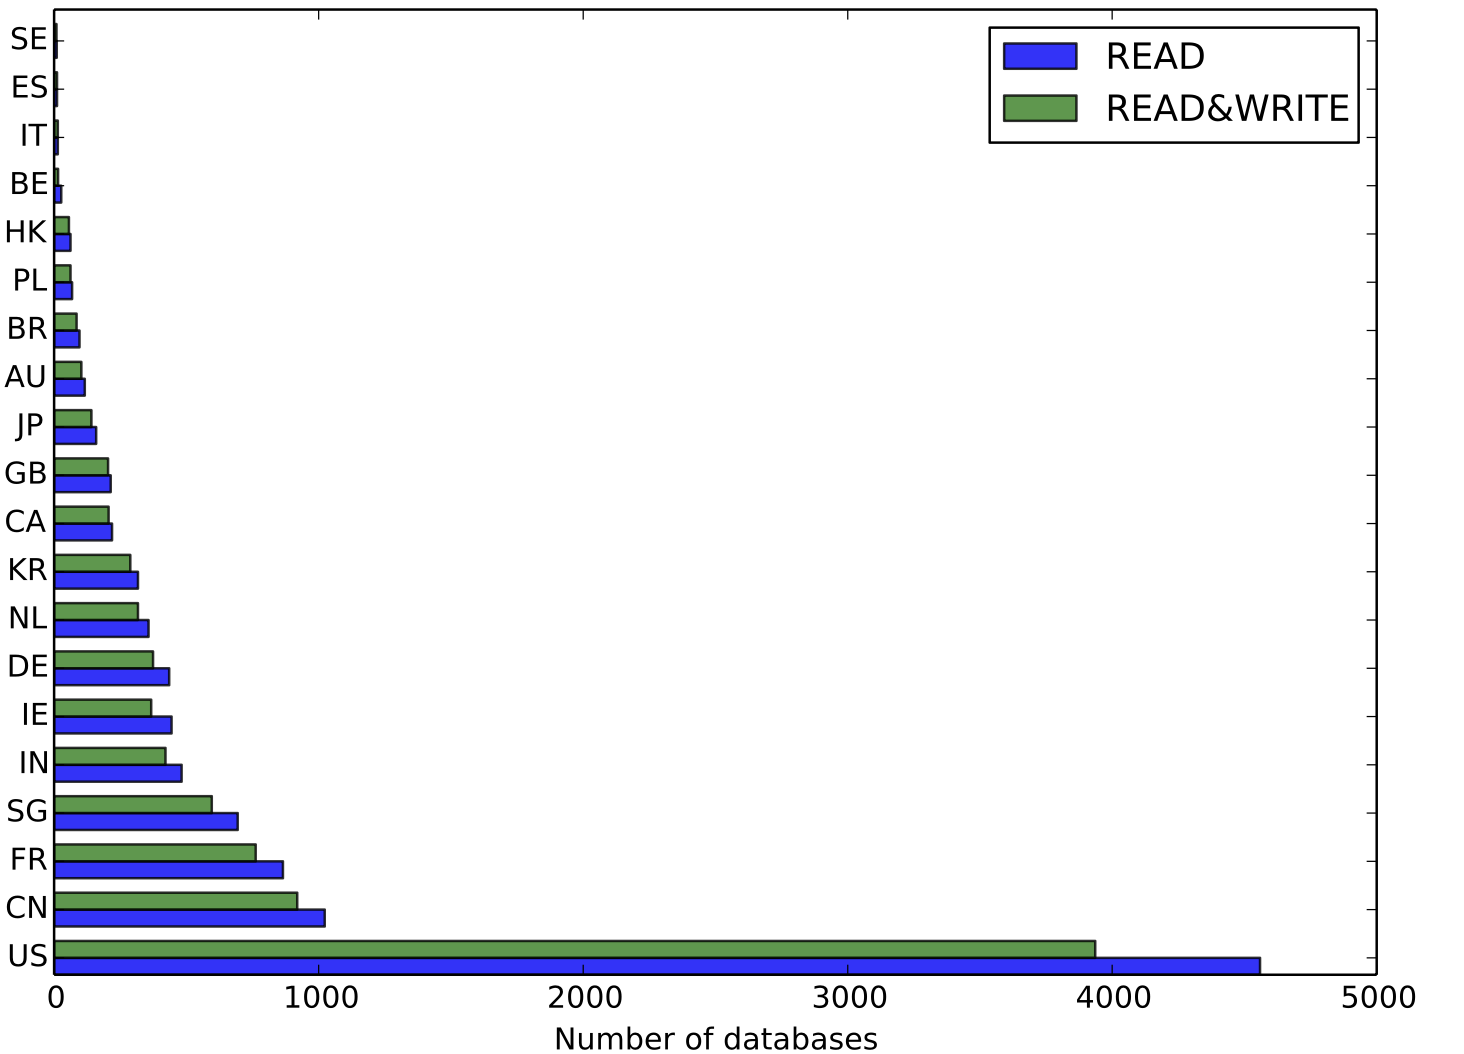
\includegraphics[width=0.5\textwidth]{res/fig3.png}
    \caption{۲۰ رتبه اول دیتابیس‌‌های استفاده شده در مناطق جغرافیایی مختلف}
    \label{fig: diagram}
\end{figure}


\subsection{بررسی‌های امنیتی}

فاز اصلی و عملی این تحقیق می‌باشد. به گونه‌ای که به سه وظیفه برای جست و جوی
نمونه‌های باز دیتابیس‌های NoSQL انجام گرفته است:

\begin{enumerate}
    \item ساخت یک نمونه یا Instance از دیتابیس مربوطه برای اتصال به آن و
    بررسی‌های اولیه ورود بدون احراز هویت
    \item بررسی و ورود به داده‌ها برای دریافت اطلاعات بدون دسترسی به محتوای اصلی
    آنها برای اثبات انتشار داده‌های حساس کاربران
    \item در معرض دید عموم قرار گرفتن سرویس‌های وب
\end{enumerate}


\subsubsection*{بررسی و نمونه‌گیری از دیتابیس جهت اتصال و انجام عملیات}

برای هر یک از آدرس‌های IP که در مرحله قبل بدست آورده شد، این فریمورک یک نمونه به
ازای هر سرویس NoSQL ایجاد می‌کند تا ضعف پیکربندی را مورد بررسی قرار دهد.

در ابتدا این ابزار در دیتابیس‌های مذکور لاگین کرده و سطوح دسترسی
\footnote{\lr{Access permission}} آنها را مورد بررسی قرار می‌دهد. اگر این ابزار
نتواند به صورت مستقیم مجوز‌های خواندن و نوشتن کاربران تعریف شده در دیتابیس را
دریافت کند وارد استراتژی دوم شده و یک workspace جدید در دیتابیس افشا شده ایجاد
می‌کند. اگر نتیجه ایجاد این workspace موفقیت آمیز بود این بدین معناست که این
دیتابیس دسترسی نوشتن را برای تمام کاربران چه داخلی و چه خارج از سیستم دارد. بعد
از این ایجاد این workspace ابزار سعی می‌کند که یک پیام هشدار برای صاحبان دیتابیس
ایجاد کند در این پیام در مورد پیکربندی اشتباه و ضعیف این نمونه توضیح خواهد داد و
صاحبان دیتابیس را با این پروژه آشنا می‌کند که قصد هیچ تخریب اطلاعاتی ندارد بلکه
می‌خواهد آنها را از بابت این نقص‌ها با خبر سازد که هر چه زودتر با سیاستی مناسب
از این دسترسی‌ها به کاربران خارج از سیستم جلوگیری انجام شود.

\subsubsection*{بررسی نشت داده}

برای بررسی نشت اطلاعات، اگر ابزار بتواند بررسی کند که دسترسی خواندن را دارد که
آن را اعلام می‌کند در غیر این صورت به صورت مستقیم به دیتابیس متصل شده و تمام متا
دیتا‌ها از قبیل ورژن کنونی دیتابیس، نقش‌های کاربران تعریف شده در دیتابیس و
همچنین نام تمام تسون‌ها (ویژگی‌های داده) را دریافت می‌کنند. لازم به ذکر است که
این ابزار این داده‌ها را با استفاده از توابع داخلی دیتابیس مانند استفاده از
\lr{Regular Expresion} توابع شمارشی و غیر بدست می‌آورد که هیچ داده‌ای از کاربران
را در ابزار تجزیه و تحلیل نکند. این داده‌ها از قبیل آدرس ایمیل، حساب‌های
شبکه‌های اجتماعی، شماره تلفن‌ها شماره حساب‌ها و گذرواژه هستند. این نتیجه مقادیر
این داده‌ها را می‌توانید در جدول ۲ مشاهده کنید.

\subsubsection*{بررسی در معرض دید قرار گرفتن سرویس‌های وب}


در این مرحله پتانسیل احتمال آسیب پذیری سرور افشا شده در برابر حمله‌های مبتنی بر
وب مورد بررسی قرار گرفته است. در عمل با استفاده از ابزاری به نام VirusTotal
آدرس‌های IP با دسترسی عمومی را وارد این برنامه کرده و تمام وب سایت‌هایی که روی
این IP مستقر شده اند را بر می‌گرداند. در نهایت محققان به این نتیجه رسیدند که
ممکن است بر روی نمونه دیتابیس NoSQL مستقر شده روی یک IP با دسترسی عمومی، وب
سایت‌ مربوط به این نمونه‌ها نیز مستقر شده باشد. اگر وب سایت به صورت عمومی از این
روش در دسترس همه افراد باشد (با ارسال درخواست به سمت این وب سایت‌ها وضعیت
درخواست شما ۲۰۰ خواهد بود.) محققان به این نتیجه رسیدند که می‌توانند از طریق این
اتصال بین وب سایت و دیتابیس به منابع دیگر آنها دسترسی داشته باشند.

\begin{LTR}
    \begin{table}[!h]
        \centering
        \begin{RTL}
            \caption{آنالیز نشت محتوای حساس}
        \end{RTL}
        \scalebox{0.5}{
            \begin{tabular}{|c|l|ccc|c|}
                \hline
                Category & FileType & MongoDB & Elasticsearch & cassandra & Total No. \\ \hline
                \multirow{9}{*}{Text/Data}
                & .log & 350,243 & 69,965,613 & 3,322 & 70,319,178 \\
                & .zip & 8,790,301  & 181,745 & 335 & 8,972,381 \\
                & .json & 7,068 & 5,612,072 & 7,413 & 5,689,553 \\
                & .xml& 2,040,533 & 981,233 & 4,480 & 3,026,246 \\
                & .txt & 150,379 & 1,459,495 & 1,733 & 1,611,607 \\
                & .pdf & 811,003 & 756,518 & 10,096 & 1,577,617 \\
                & .text & 27,219 & 443,990 & 132 & 471,341 \\
                & .gz & 6,416 & 191,387 & 132 & 14,426 \\
                & .docx & 18,910 & 45,375 & 824 & 65,109 \\
                \hline
                \multirow{6}{*}{Image/Video}
                & .jpg & 22,772,623 & 25,267,934 & 739,508 & 48,780,065 \\
                & .png & 4,558,372 & 6,072,558 & 112,561 & 10,743,491 \\
                & .jpeg & 613,202 & 707,461 & 34,348 & 1,355,121 \\
                & .gif & 594,428 & 581,382 & 1,926 & 1,335,121 \\
                & .mp4 & 429,038 & 470,231 & 4,333 & 903,602 \\
                & .webp & 39,994 & 75,163 & 249,609 & 364,766 \\
                \hline
                \multirow{4}{*}{Code}
                & .html & 1,618,010 & 11,684,183 & 272,883 & 13,575,076 \\
                & .ts & 8,383 & 335,539 & 11,132 & 355,054 \\
                & .js & 58,213 & 135,167 & 1,898 & 195,278 \\
                & .hll & 47 & 585 & 0 & 632 \\ \hline
                File Keys & .key & 10,444 & 10,832,464 & 2,620 & 10,845,528 \\ \hline
                \multirow{3}{*}{Crypto Files}
                & .pem & 247 & 130,370 & 13 & 130,630 \\
                & .pfx & 89 & 1,258 & 4 & 1,351  \\
                & .p12 & 31 & 457 & 7 & 495 \\ \hline
                DB & .sql(Dumlps) & 2,270 & 237,306 & 186 & 239,762 \\ \hline
                Backup & .bak & 1,487 & 5,364 & 300 & 7,151 \\ \hline
                Password & .kbd(Keepass) & 10 & 42 & 0 & 52 \\ \hline
            \end{tabular}
        }
    \end{table}
\end{LTR}

\newpage

\section{آزمایش‌ها و تحلیل نتایج}

در‌ این قسمت به نحوه عملکرد کلی فریمورک توسعه داده شده توسط محققان می‌پردازیم.
همان طور که بالاتر بارها اشاره شد، این فریمورک طی تمام آزمایش‌ها، محققان اصلا
ماهیت داده‌های دیتابیس و محتوای آنها را مورد بررسی قرار نداده بلکه تماما روی
دسترسی در استفاده از داده‌ها تاکید زیاد داشتند.

در این بخش با نمایش یک نمونه کد، به طور کلی در مورد نحوه عملکرد این فریمورک صحبت
خواهیم کرد.

\begin{LTR}
    \begin{lstlisting}
        # Connect to the database
        mongo_client.connect(ip_address)
        # Get database names
        db_names = list_database_name()
        # Mongo-shell method used to get role mappings
        db.getRoles(showBuiltinRoles: false)
        # Get collection names
        collections = list_collection_names()
        # Map-reduce function used to get field-mapping for each table
        map = Code("function() {
            for (key in this) {
                emit(key, null);
            }
        }")
        reduce = Code("function(key, stuff) { return null; }")
        results = collection.map_reduce(map, reduce, "myresults")
        # Query methods for field and object detection
        count({ fieldname: {"$exists": True} })
        count({ fieldname: {r'.*\.(fieldvalue)'} })
        # Write the message in a new database
        writedb = mongo_client[MONGO_DB]
        writecollection = writedb[MONGO_COLLECTION]
        writecollection.insert_one(MONGO_DOC)
    \end{lstlisting}
\end{LTR}

\subsection{بررسی قسمتی از فرایند مطرح شده}

در خط ۲ با استفاده از آدرس IP حاضر در لیست آدرس‌ها، قصد اتصال به دیتابیس مانگو
را به صورت ریموت داریم. سپس بعد از اتصال موفق می‌توانیم با استفاده از واسط
\lr{Mongo Shell} دستوراتی را برای انجام عملیاتی روی دیتابیس مورد نظر انجام دهیم.
برای مثال در خط بعدی آن نام تمام دیتابیس‌هایی که در این آدرس IP وجود دارد را
دریافت می‌کنیم و در متغیر dbnames قرار می‌دهیم. با استفاده از این عمل یعنی عاملی
که توانسته به دیتابیس متصل شود قادر به خواندن محتوا بوده است که در این جا با
اطمینان اعلام می‌کنیم که دسترسی خواندن در این دیتابیس برای یک کاربر عادی و خارج
از سیستم وجود دارد. بعد از آن با استفاده از متد \lr{getRoles} می‌توانیم تمام
کاربرانی که در این دیتابیس تعریف شده‌اند براساس سطح دسترسی آنها، را دریافت کنیم.
برای دسترسی به جداول (اصطلاحا در دیتابیس‌های مانگو به آن کالکشن می‌گویند.) از
تابع که نوشته‌ایم استفاده کردیم تا لیست تمام کالکشن‌های مروبط به یک دیتابیس را
دریافت کنیم. برای آن که بتوانیم فیلد‌های (کلید‌های) مربوط به یک کالکشن
(مجموعه‌ای از داکیومنت‌ها) را دریافت کنیم از یک تابع Map-Reduce استفاده کردیم که
تنها نام کلید‌های استفاده شده در این کالکشن را به ما برگرداند که بدایم دیتابیس
شامل چه فیلد‌هایی است. در نهایت با استفاده از Regex توانستیم تمام داده‌های مربوط
به متادیتا هر کالکشن را توسط الگوی "exists" برای تشخیص تعداد فیلد‌ها جست و جو
کنیم. در سه خط کد آخر می‌توان متوجه شد که ما می‌خواستیم که از داشتن دسترسی نوشتن
در دیتابیس اطمینان حاصل کنیم که به همین خاطر سعی کردیم نتیجه تحقیقات خود را در
یک کالکشن جدید در همان دیتابیس به عنوان یک داکیومنت جدید اضافه کنیم.

\subsection{یادآوری تابع Map-Reduce \cite{officialMapReduce}}

تابع Map-Reduce یک تابع دلخواه و قابل سفارشی‌سازی توسط برنامه‌نویس در زبان جاوا
اسکریپت است (اساس کلی دیتابیس‌های مانگو بر پایه موتور NodeJS و زبان Javascript
می‌باشد.) که به واسطه آن عملیات مختلفی مانند بدست آوردن کلید‌های استفاده شده در
یک داکیومنت، گروه‌بندی اجزا و یا دستکاری روی گروه‌بندی اجزا با استفاده از توابعی
مانند \lr{sum()} یا \lr{count()} می‌باشد.

\begin{LTR}
    \begin{lstlisting}
        db.cardata.find()
        { "_id": ObjectId("9dd74a***2340***"), "name": "Peugeot", "Series": "2", "qty": 10 },
        { "_id": ObjectId("5f94********"), "name": "BMW", "Series": "X", "qty": 112 },
        { "_id": ObjectId("2e127a********"), "name": "Peugeot", "Series": "5", "qty": 105 },
        { "_id": ObjectId("8m113********"), "name": "BMW", "Series": "M", "qty": 25 },

        var map = function() { emit(this.name, this.qty) }
        var reduce = function(key, value) { return Array.sum(values) } 
        db.cardata.mapreduce(map, reduce, "myResults")
        db.myResults.find()
        { "_id": "BMW", "value": 137 },
        { "_id": "Peugeot", "value": 115 }
    \end{lstlisting}
\end{LTR}

\subsection{بررسی در انواع دیتابیس‌های اشاره شده}

دقیقا همانند کد بالا در دو دیتابیس \lr{Cassandra} و \lr{Elasticsearch} به شکل
مناسب برای انجام همان فرایند‌ها، عملیات مورد نظر را اعمال کردیم اما در دیتابیس
مموری Redis به شکل قبلی نتوانستیم عمل کنیم چرا که نمی‌توانستیم به طور مستقیم
برخلاف سرویس‌های قبلی صحت دسترسی به لیست‌ها و کالکشن‌ها را بررسی کنیم. (این
ویژگی در نسخه ۶ به بعد معرفی شد به گونه‌ای که در این مقاله امکانش میسر نبوده
است). همچنین از آنجایی که در دیتابیس Redis نمی‌توان تعداد آبجکت‌ها و فیلد‌ها را
بدست آورد (به دلیل key:value بودن) از انجام این عملیات جلوگیری کرده‌ایم چرا که
برای بدست آوردن هر فیلد ممکن بود که بتوانیم به مقدار آن فیلد دسترسی داشته باشیم
که این قوانین ما را نقض می‌کند. در نهایت برای عدم آسیب رساندن به بقیه داده‌ها
سعی کردیم یک کلید جدید ایجاد کنیم و پیام هشدار خود را در آن ایجاد کنیم. در زیر
می‌توانید عملیات (کلی) انجام شده در دیتابیس Redis را بررسی کنید.

\begin{LTR}
    \begin{lstlisting}
        # Connect to the database
        r = redis.Redis(ip_address)
        # Get key names
        keys = r.keys(pattern=u'*')
        # Get eventual number of occurrences of key fieldnames
        occurrences = scan_iter(match="fieldname")
        for match in occurrences:
            counter += 1
        # Write the warning message
        r.append(key, value)
    \end{lstlisting}
\end{LTR}

نتایج بدست آمده بر اساس آزمایشاتی که در بالاتر توضیح داده شد به تفکیک سرویس‌های
NoSQL به طور دقیق در این بخش بررسی می‌شود. به طور کل ۶۷ میلیون آدرس IP برای این
تحقیق جمع‌آوری شده است بطوری که سهم هر سرویس از این آدرس‌های IP در جدول ۳ آمده
است.

\begin{LTR}
    \begin{table}[h]
        \centering
        \begin{RTL}
            \caption{آدرس‌های IP یافت شده بین بازه اکتبر ۲۰۱۹ تا مارچ ۲۰۲۰}
        \end{RTL}
        \scalebox{1}{
            \begin{tabular}{|c|c|}
                \hline
                NoSQL Service name & IP Address Quantitiy \\ \hline
                AmazonEC2 & 41,245,648 \\ \hline
                AzureCloud & 13,712,761 \\ \hline
                Google Cloud & 7,346,944 \\ \hline
                OVH & 3,019,008 \\ \hline
                TencentCloud & 1,383,664 \\ \hline
                DigitalOcean & 1,007,616 \\ \hline
            \end{tabular}
        }
    \end{table}
\end{LTR}

\begin{figure}[H]
    \centering
    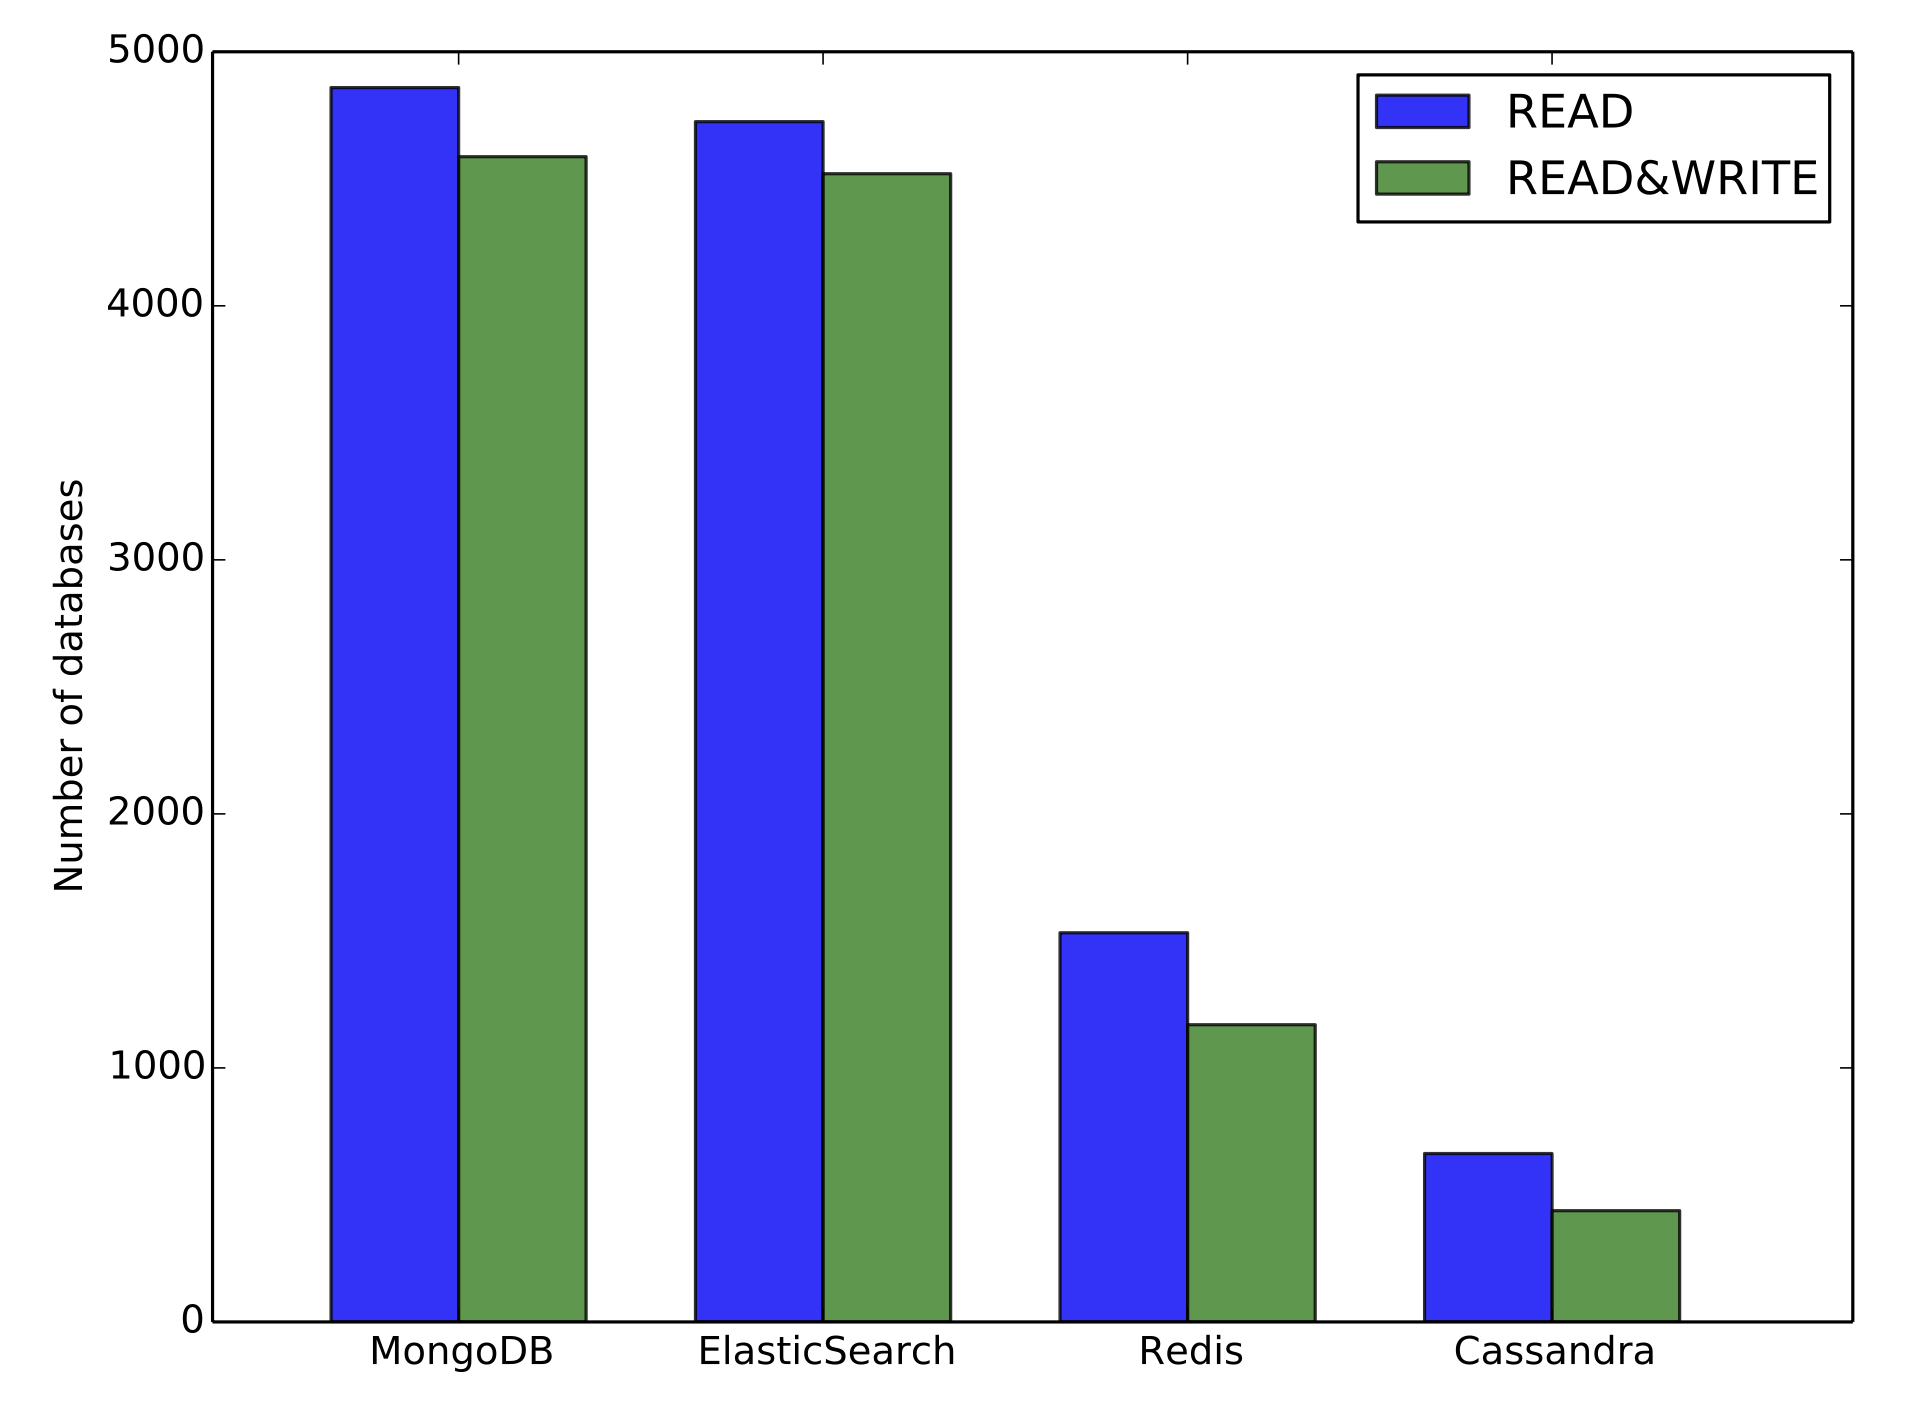
\includegraphics[width=0.5\textwidth]{res/a.png}
    \caption{بررسی پیکربندی سرویس‌های مختلف NoSQL}
    \label{fig: diagram}
\end{figure}

\subsection{توزیع دیتابیس‌های NoSQL به تفکیک پارامتر‌های مختلف}

\begin{LTR}
    \begin{table}[h]
        \centering
        \begin{RTL}
            \caption{تعداد سرویس‌های افشا شده NoSQL}
        \end{RTL}
        \scalebox{0.8}{
            \begin{tabular}{|c|cccc|c|}
                \hline
                Misconfiguration & MongoDB & Elasticsearch & Redis & Cassandra & TotalNo. \\ \hline
                Read & 4,859 & 4,735 & 1,532(2,029) & 663 & 12,276 \\
                Read Only & 272 & 205 & 362 & 225 & 1,064 \\
                Read \& Write & 4,587 & 4,520 & 1,170 & 438 & 10,715 \\ \hline
            \end{tabular}
        }
    \end{table}
\end{LTR}

با توجه به نمودار شکل ۲ می‌توان دریافت که محبوبیت استفاده از دیتابیس‌های MongoDB
نسبت به Cassandra بسیار زیاد است. (البته بر اساس آمار بدست آمده در سایت
db-engines.com از سال ۲۰۲۰ تا نوامبر ۲۰۲۳) به همین خاطر کمتر توسعه دهنده یا
شرکتی وجود دارد که از دیتابیس Cassandra استفاده کند. در نمودار شکل ۳ می‌توان
متوجه شد که بیشتر توسعه دهندگان علاقه زیادی به استفاده از سرویس‌های ابری دارند
که از دیتابیس‌های NoSQL پشتیبانی می‌کنند. همانطور که می‌توانید مشاهده کنید سرویس
AmazonEC2 بیشترین میزان ضعف پیکربندی را در بین تمام سرویس‌ها داشته است (به تعداد
۵،۵۶۸ سرویس دیتابیسی). همچنین در نمودار شکل ۴ می‌توانید تعداد دیتابیس‌های NoSQL
را به تفکیک کشور‌های مختلف مشاهده کنید. همانطور که انتظار می‌رفت بیشتر سرویس‌ها
در ایالت متحد آمریکا مستقر شده‌اند  که بیشترین مقدار تعداد افشای دیتابیس را در
بین تمام کشور‌ها دارند تقریبا ۴۴/۶٪ را به خودش اختصاص می‌دهد.

\begin{figure}[H]
    \centering
    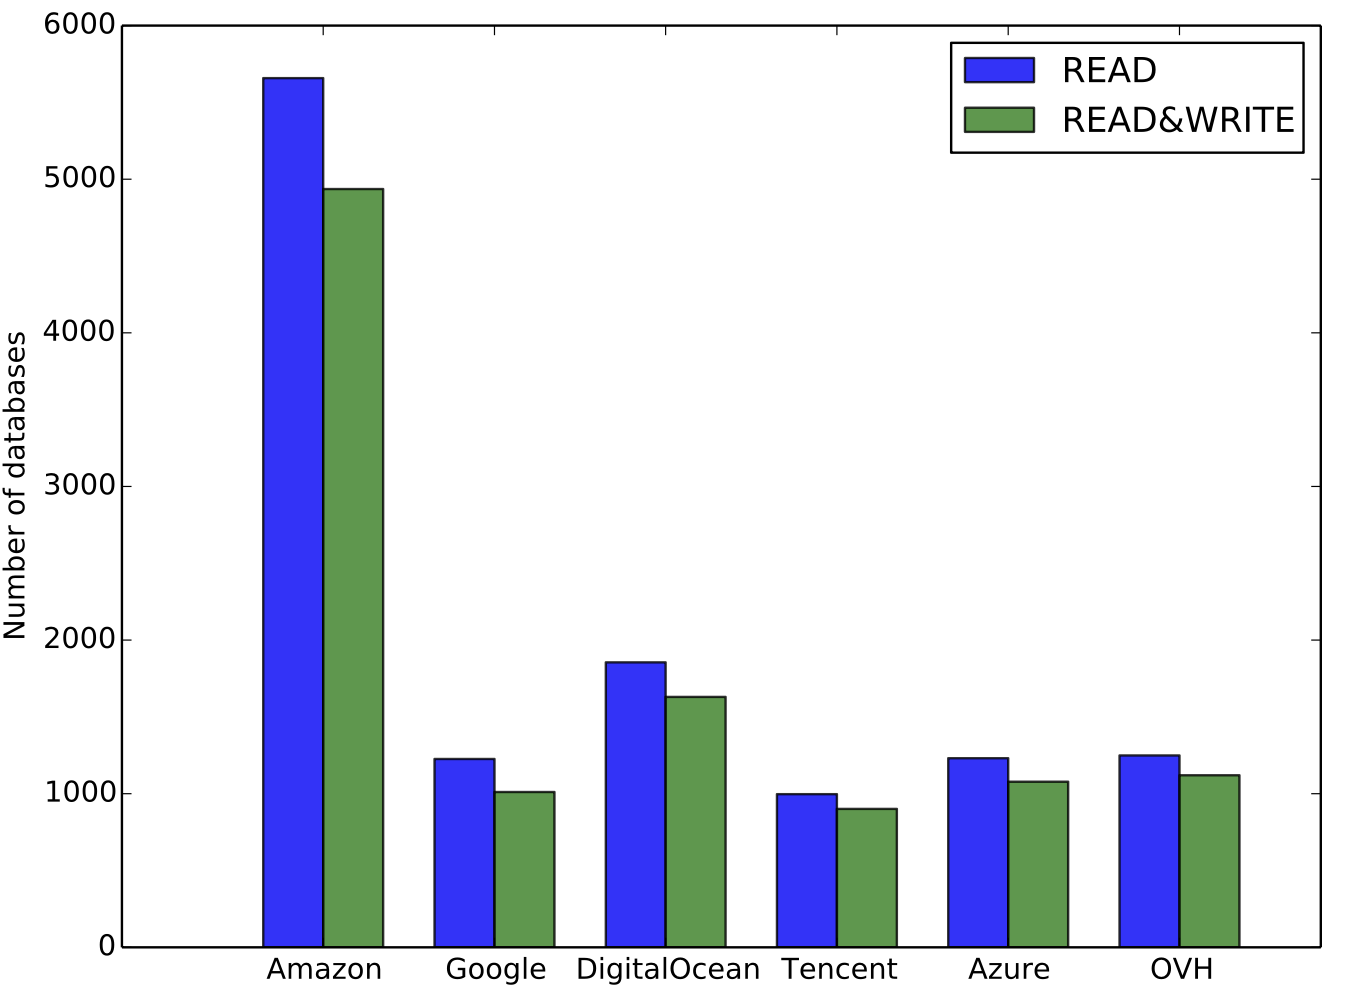
\includegraphics[width=0.5\textwidth]{res/b.png}
    \caption{بررسی ضعف پیکربندی دیتابیس‌های NoSQL در سرویس‌های ارائه دهنده خدمات ابری}
    \label{fig: diagram}
\end{figure}

\subsection{بررسی معیار کیفی دیتابیس‌های فاش شده}

در طی گزارشی که در مورد این مقاله می‌نوشتم همواره سوالی که در ذهنم وجود داشت این
بود که چه معیاری برای بررسی کیفیت داده‌ها در طی این همه فرایند بررسی و تحقیق
وجود داشته است؟ در این قسمت به بررسی این سوال می‌پردازیم. اما در کوتاه‌ترین جواب
می‌توان گفت که تعداد زیادی از این دیتابیس‌های فاش شده در سرویس‌های NoSQL تنها
برای آزمایش توسط برنامه‌نویسان بوده است نه همه برای استفاده در اپلیکیشن‌های بزرگ
نهایی در دست کاربران!

معیار اصلی برای سنجش کیفیت دیتابیس‌های فاش شده بر اساس حجم دیتابیس‌ها و متادیتای
مربوط به جداول و فیلد‌ها می‌باشد. اینکه هر چقدر دیتابیس سنگین‌تر باشد به معنای
آن است که احتمالا شامل جداول بسیار زیاد و داده‌های مختلف در آن می‌باشد. تعدادی
از دیتابیس‌ها به حجم چند مگابایتی می‌رسیدند که بیشتر در آنها از کلماتی مانند
Test استفاده شده بود یا اینکه کلا خالی بودند. محققان این اطلاعات را از طریق
توابعی متنوعی که در هر سرویس دیتابیسی ارائه می‌شود (استفاده از درایور‌هایی مانند
pymongo و غیره) دست یافتند. همانطور که در قسمت ردیس گفته شد، در این دیتابیس (در
نسخه‌ای که این مقاله نوشته شده است) نمی‌توان به این اطلاعات بدون نشت و دیدن
داده‌ها، دست یافت.

\subsubsection{دیتابیس Mongo}

میانگین اندازه حجم این دسته از دیتابیس‌های فاش شده به مقدار $ 299 \pm 40 $
مگابایت می‌رسید که بیشتر از ۲۷۱ دیتابیس (۵/۵٪) به اندازه بیشتر از ۱۰۰ مگابایت
می‌رسند.  تعداد ۹۳ نمونه از این دیتابیس‌ها که حدودا (۱/۹٪) را شامل می‌شد اندازه
حجم بیشتر از ۵۰۰ مگابایت را داشتند. بین این بررسی، ۴۴۵ (۹/۱٪) حاوی کلمه test به
عنوان نام کالشن‌ها بودند که تعداد ۲۶۲ نمونه از آنها (۵/۳٪) دارای اندازه حجم کمتر
از ۱ مگابایت بودند.

\subsubsection{دیتابیس Elasticsearch}

میانگین اندازه حجم این دیتابیس‌ها به طور کلی $ 109.04 \pm 422.57 $ مگابایت بوده
است. این دیتابیس نسبت به MongoDB حجم بیشتری از داده‌ها را نگهداری می‌کردند. ۶۵۲
نمونه از این دیتابیس‌ها (۱۳/۷٪) اندازه حجم بیشتر از ۱۰۰ مگابایت را داشتند. ۲۳۹
نمونه‌ دیگر (۵/۲٪) اندازه حجم بیشتر از ۵۰۰ مگابایت را داشتند و در نهایت در این
بررسی بیشتر از ۶۶۱ نمونه دارای کلمه test در نام اندیس‌هایشان بودند که ۱۲۰ نمونه
از آنها حجم کمتر از ۱ مگابایت داشتند.

\subsubsection{دیتابیس Redis}

در این دیتابیس ۱۰۱ نمونه از کلمه test به عنوان نام کلید مورد نظر استفاده کرده
بودند.

\subsubsection{دیتابیس Cassandra}

میانگین اندازه حجم این دیتابیس به اندازه $ 10.78 \pm 33.61 $ مگابایت بوده است.
۲۱ دیتابیس (۳/۱٪) اندازه حجم بیشتر از ۱۰۰ مگابایت داشتند. همچنین ۱۸۰ دیتابیس
(۲۶/۵٪) از کلمه test به عنوان نام جدول استفاده کرده بودند و در نهایت ۴۵ نمونه از
آنها (۶/۶٪) کمتر از ۱ مگابایت اندازه حجمشان بود. 

\subsection{بررسی محتوای فاش شده}

در جدول ۲ می‌توانید انواع فایل‌هایی که در این تحقیق در این ۴ دیتابیس فاش شده‌اند
را مشاهده کنید. اما نکته جالب آن است که بیشترین مقدار یافت شده در مورد لاگ‌ها
می‌باشد مخصوصا در دیتابیس Elasticsearch. چرا که برخی شرکت‌ها برای راه‌اندازی یک
سیستم مانیتورینگ ساده از ابزار‌هایی مانند Kibana، Grafana، Elasticsearch و
Logstash استفاده می‌کنند. برای نگهداری داده‌های مربوط به یک برنامه مانیتورینگ از
دیتابیس Elasticsearch استفاده می‌شود و برای مدیریت و ذخیره‌سازی لاگ‌ها به صورت
بحران‌های زمانی \footnote{\lr{Time Series Databases}} از ابزار logstash استفاده
می‌شود. ۴۵۲ نمونه از دیتابیس Elasticsearch که شامل ۹/۵٪ از کل دیتابیس‌های تحقیق
شده می‌باشد از فایل‌های .log استفاده می‌کنند که مقدار این نوع از فایل‌ها ۵۰٪ از
داده‌ها را تشکیل می‌دهد. مابقی داده‌ها با فرمت‌های jpg png jpeg git mp4 webp نیز
به عنوان فایل‌های چندرسانه‌ای در این دیتابیس یافت شده است. در نمودار شکل ۴
می‌توانید درصد استفاده از دیتابیس‌ها از ۴ دسته‌بندی داده متنی، رسانه‌ای، کد و
داده‌های حساس مانند نام کاربری، گذرواژه و حتی فایل‌های امنیتی وب را مشاهده کنید.

در همین راستا، محققان برای پیدا کردن داده‌های حساس‌تر روی فیلد‌های نام‌کاربری،
گذرواژه و شماره تلفن در دیتابیس‌های Elasticsearch، MongoDB و Cassandra تحقیقاتی
انجام دادند. علاوه‌بر این آنها به دنبال فیلد‌های مخصوصی مانند حساب‌های کاربری در
شبکه‌های Linkedin و Facebook گشتند. نتیجه این قسمت را می‌توانید در جدول ۵ مشاهده
کنید. 

\begin{figure}
    \centering
    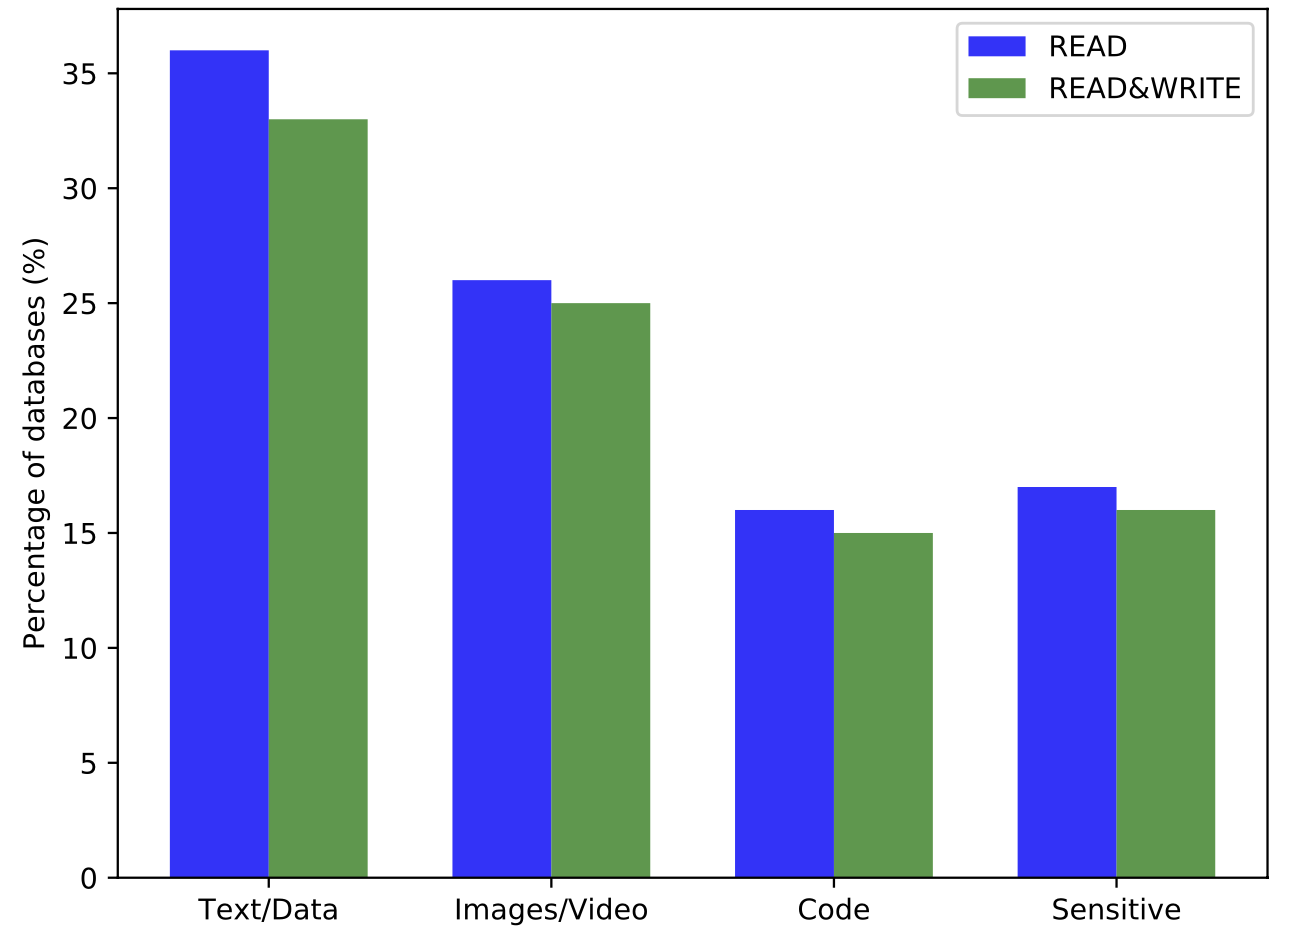
\includegraphics[width=0.5\textwidth]{res/fig4.png}
    \caption{درصد موجودیت داده‌های حساس دیتابیس‌ها در ۴ دسته‌بندی ذکر شده}
    \label{fig: diagram}
\end{figure}

برای بررسی دقیق‌تر نشت داده‌هایی مانند ایمیل و شماره تلفن کاربران، محققان یک
آستانه بین ۱۰۰ تا ۱۰۰۰ داده بین تعدادی از آدرس‌های ایمیل و شماره تلفن قرار
دادند. بررسی آن در نمودار شکل ۶ آمده است. از آن می‌توان نتیجه گرفت که بین تمام
دیتابیس‌های یافت شده در این بررسی تعداد کمی از آنها شامل داده‌هایی برای فیلد‌های
آدرس ایمیل و شماره تلفن هستند.

% TODO: Should fix sentences (Double check at the end)

برای مثال در بین ۱،۱۲۶ دیتابیس MongoDB تنها ۱۵۱ دیتابیس دارای فیلد ایمیل هستند
که بیشتر از ۱۰۰ داده در رابطه با ایمیل دارند و ۸۳ دیتابیس دیگر بیشتر از ۱۰۰۰
داده. 

در ۸۵۲ دیتابیس Elasticsearch در رابطه با فیلد آدرس ایمیل، تنها ۴۰۴ دیتابیس بیشتر
از ۱۰۰ داده ایمیل دارند و ۲۰۶ دیتابیس دیگر بیشتر از ۱۰۰۰ ایمیل دارند.

همچنین در ۴۵ دیتابیس Cassandra فقط ۲۵ دیتابیس بیشتر از ۱۰۰ داده ایمیلی دارند و
۱۲ دیتابیس دیگر بیشتر از ۱۰۰۰ داده ایمیلی را شامل می‌شوند.

\begin{figure}
    \centering
    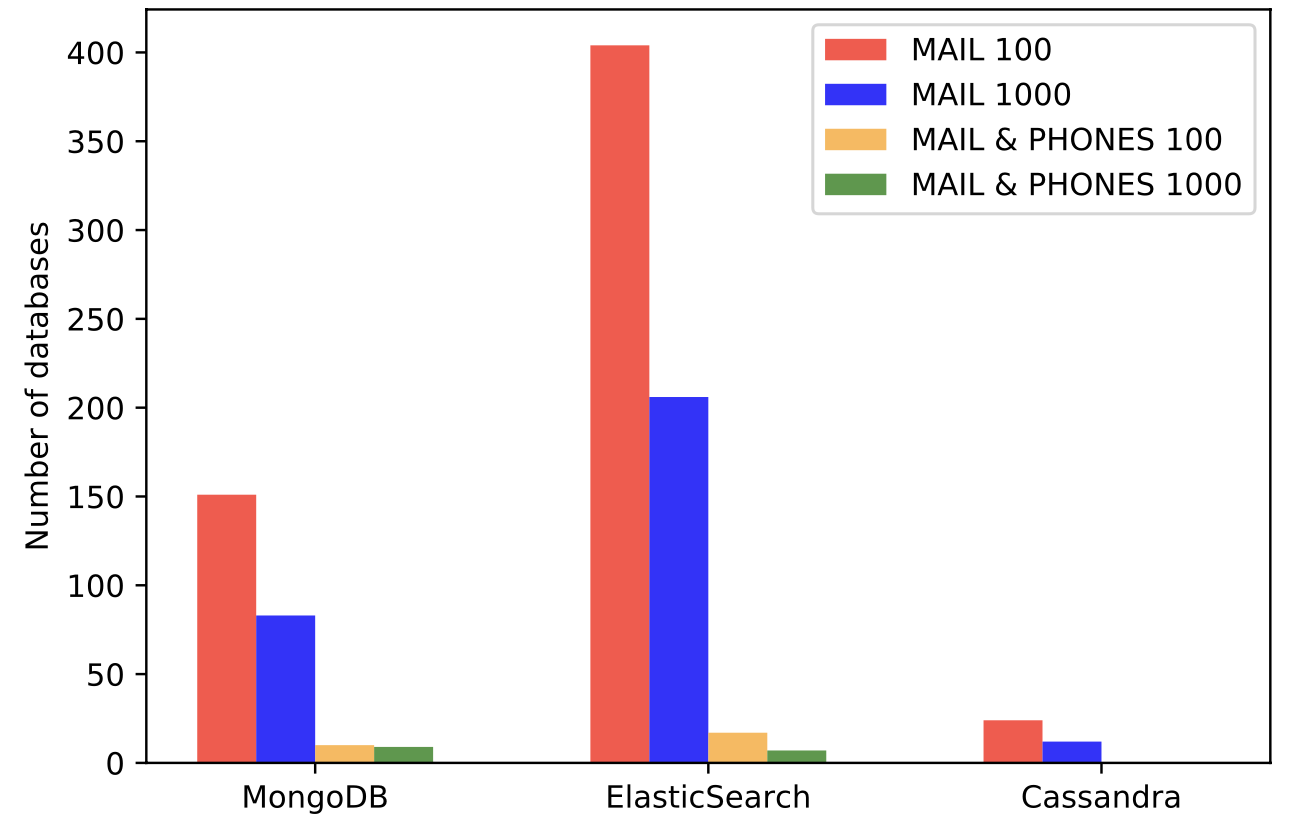
\includegraphics[width=0.5\textwidth]{res/fig5.png}
    \caption{بررسی نشت داده، بین آستانه ۱۰۰ و ۱۰۰۰ ایمیل و شماره تلفن}
    \label{fig: diagram}
\end{figure}

\begin{LTR}
    \begin{table}[h]
        \centering
        \begin{RTL}
            \caption{آنالیز و بررسی پتانسیل نشت پذیری داده‌های حساس کاربران}
        \end{RTL}
        \scalebox{0.8}{
            \begin{tabular}{|c|cc|cc|cc|}
                Fields & \multicolumn{2}{c}{\textbf{Elasticsearch}} & \multicolumn{2}{c}{\textbf{Cassandra}} & \multicolumn{2}{c}{\textbf{MongoDB}} \\ \hline
                & No.Databases & No.resources & No.Databases & No.resources& No.Databases & No.resources \\ \hline
                E-mail & 852 & 2,189,078 & 45 & 210,244 & 1,126 & 2,715,765 \\ \hline
                Password & 69 & 94,647 & 9 & 19 & 147 & 208,343 \\ \hline
                Phone Number & 68 & 167,234 & 5 & 34 & 51 & 654,634 \\ \hline
                Nominative & 236 & 2,274,327 & 20 & 13,168 & 270 & 1,248,592 \\ \hline
                Facebook & 266 & 221,576 & 40 & 623 & 84 & 34,772 \\ \hline
                Linkedin & 133 & 26,695 & 6 & 497 & 39 & 15,089 \\ \hline
            \end{tabular}
        }
    \end{table}
\end{LTR}

\subsection{افشای وب سرویس‌ها}

همانطور که می‌دانید دیتابیس‌ها داده‌های مربوط به سایت‌ها و اپلیکیشن‌های مختلفی
را نگهداری می‌کنند. در صورتی که یک هکر بتواند وارد این دیتابیس‌ها شود با
دسترسی‌های خواندن/نوشتن می‌تواند داده‌های دیتابیس این اپلیکیشن‌ها را تخریب کند
یا در بدترین حالت می‌تواند موجب تغییر چهره \footnote{Deface} آن وب سایت یا
اپلیکیشن شود که در نهایت موجب انتشار داده‌های نامناسب و غیر معتبر خواهد شد.
محققان توانستند با بررسی آدرس‌های IP و تبدیل آنها به آدرس‌های معنادار DNS به
وب‌سایت‌هایی برسند که ممکن است آن وب‌سایت‌ها از این دیتابیس‌ها خوراک
\footnote{Feed} دریافت کنند. نتیجه دسترسی به این وب‌سایت‌ها در جدول ۶ آمده است.
(نتیجه تنها روی وب‌سایت‌هایی بوده است که در حین تحقیق قابلیت دسترسی داشتند و
بدون request timeout محققان می‌توانستند به آنها دسترسی داشته باشند). ۲۹۱ وب‌سایت
به وسیله دیتابیس MongoDB، ۳۳۴ وب‌سایت به وسیله دیتابیس Elasticsearch، ۲۷ مورد
برای دیتابیس Redis و ۱۱ مورد برای دیتابیس Cassandra که به ترتیب ۱۶/۸٪، ۱۹/۳٪
۱/۵٪ و ۰/۶٪ وب‌سایت‌هایی به صورت عمومی در دسترس بودند.

به طور کلی، با دسترسی هکر به یک دیتابیس دو نوع از حمله می‌تواند رخ دهد:

\begin{enumerate}
    \item حلمه به روش تخریب چهره \footnote{Defacement}
    \item حمله به روش تزریق کد \footnote{\lr{Code injection}}
\end{enumerate}

\begin{LTR}
    \begin{table}[h]
        \centering
        \begin{RTL}
            \caption{افشای وب سرویس‌ها: لیست تعداد سایت‌هایی که محققان توانستند از آن پاسخ بگیرند}
        \end{RTL}
        \scalebox{0.8}{
            \begin{tabular}{|c|c|c|}
                \hline
                Http code & No. Websites & Summary \\ \hline
                200 & 1,723 & Request Successed \\ \hline
                302 & 473 & Found, URI changed temporary \\ \hline
                404 & 244 & Not Found \\ \hline
                403 & 136 & Forbidden \\ \hline
                301 & 105 & Moved Permanently \\ \hline
                401 & 84 & Unauthorized \\ \hline
                502 & 53 & Bad Gateway \\ \hline
                307 & 49 & Temporary Redirect \\ \hline
                503 & 29 & Service Unavailable \\ \hline
                500 & 24 & Internal Server Error \\ \hline
                308 & 21 & Permanent Redirect \\ \hline
                400 & 19 & Bad Request \\ \hline
                203 & 16 & Request successed but not from the origin server \\ \hline
                405 & 9 & Method Not Allowed \\ \hline
                406 & 7 & Not Acceptable \\ \hline
                204 & 4 & No content \\ \hline
                504 & 3 & Gateway Timeout \\ \hline
                522 & 3 & Server Connection Timeout \\ \hline
                304 & 1 & No contnet \\ \hline
                402 & 1 & Payment required \\ \hline
                424 & 1 & Failed dependency \\ \hline
                521 & 1 & Web Server down \\ \hline
                526 & 1 & Invalid SSL certificate \\ \hline
            \end{tabular}
        }
    \end{table}
\end{LTR}

\subsubsection{حمله به روش تخریب چهره}

هکر‌ها از طریق تغییر داده‌های مربوط به دیتابیس سعی می‌کنند فضای تخریب و دزدی
اطلاعات را فراهم کنند. برای مثال تصویر یا متنی را در دیتابیس تغییر می‌دهند.
کاربران هم این داده‌ها را در صفحه وب‌سایت‌ها می‌بینند و از آنجایی که به این
صفحات اعتماد دارند فکر می‌کنند که این داده‌ها از منابع شناخته شده‌ای منتشر
می‌شود و در دام هکر‌ها می‌افتند. محققان در این تحقیق ۴۹۴ وب‌سایت که پتانسیل آسیب
پذیری و تغییر چهره برای اهداف فیشینگ داشتند را پیدا کردند چرا که اطلاعات مهمی را
داشتند و حساسیت این اطلاعات برای هکر‌ها بسیار حائز اهمیت است.

\subsubsection{حمله به روش تزریق کد}

این حمله از سناریو قبلی حتی خطرناک‌تر است. تزریق کد همانطور که از نامش پیداست
روشی است که به هکر‌ها این امکان را می‌دهند تا براساس آسیب پذیری‌هایی که در یک
سایت وجود دارد، کد جاوا اسکریپت مخصوصی را اجرا کنند و بدون داشتن مجوز اجرا در
وب‌سایت می‌توانند به صورت کامل اجرا شود و از آنجایی که دسترسی نوشتن را روی
دیتابیس دارند می‌تواند برای محتوای داخل دیتابیس خطرناک باشد. طبق این تحقیق، ۲۹۹
وب‌سایت را یافتند که پتانسیل این آسیب پذیری را دارند تا موجب تخریب اطلاعات
کاربران شود.

\subsection{آنالیز در معرض خطر بودن نمونه‌ها}

در بین تمام دیتابیس‌ها، نمونه‌های دیتابیس Redis بیشترین تعداد حمله را داشته است.
معیار محققان برای یافتن نمونه‌های در معرض خطر، در حقیقت جست و جوی کلمات مشکوک در
نام جداول بوده است.

در دیتابیس MongoDB کلماتی مانند \lr{"hacked by unistellar"} و \lr{"how to
restore"} جست و جو شده است به گونه‌ای که ۳۸۹ دیتابیس در این جست و جو پیدا کردند.

در دیتابیس Elasticsearch محققان کلمه \lr{"readme"} را جست و جو کردند که به طور
مستقیم به هکر‌های رمزنگاری و دزد اطلاعات مربوط می‌شود که در نهایت ۶۲۲ مورد از
این کلمه یافت شد.

در دیتابیس Redis محققان کلمات \lr{"crackit"}، \lr{"Back"}، \lr{"1"} و
\lr{"trojan"} را جست و جو کردند که مربوط به حمله سال ۲۰۱۸ به نمونه‌های دیتابیس
Redis در حمله سایبری بوده است \cite{openRediServer}. ۶۲۵ مورد از این کلمات در
دیتابیس Redis یافت شد.

\subsection{تجزیه و تحلیل تاثیر تحقیقات امنیتی}

در انتهای این مقاله، تاثیر این تحقیق و پروژه را مورد بررسی قرار می‌دهیم. از
اکتبر ۲۰۱۹ تا دسامبر ۲۰۱۹ محققان این پروژه را در مرحله اجرا قرار دادند. بعد از
اولین اجرای خود دوباره در ژانویه سال ۲۰۲۰ تا مارس ۲۰۲۰ این برنامه را اجرا کردند
تا بررسی کنند که آیا برنامه‌نویسان و مدیران سیستمی پیام آنها را دریافت کردند و
پیکربندی خود را به حالت امن تبدیل کردند؟ نتیجه در نمودار شکل ۷ آمده است.

در این نمودار می‌توان دریافت که از ۶۶۳ نمونه دیتابیس Cassandra ۳۱۵ نمونه یعنی
حدودا ۴۷/۵٪ دیتابیس‌ها بعد از دریافت پیام محققان پیکربندی خود را متناسب با شرایط
امنیتی تنظیم کردند و دیگر به صورت عمومی قابل دستیابی نبودند.

از ۲،۰۲۹ نمونه دیتابیس Redis، ۹۱۴ نمونه دیگر قابل ردیابی و دستیابی به صورت عمومی
نبودند به طوری که ۲۷ نمونه از آنها برای ورود به سیستمشان نیازمند احرازهویت
بودند. (تقریبا ۴۶/۳٪ آنها دیگر آسیب پذیری اولیه مانند احرازهویت را نداشتند!)

از ۴،۷۲۵ نمونه دیتابیس Elasticsearch، ۱،۵۳۹ نمونه دیگر در دسترس عموم نبودند و ۴۰
نمونه از آنها درخواست احرازهویت برای ورود به سیستم دیتابیس داشتند. (مقدار ۳۳/۴٪
از دیتابیس‌های Elasticsearch جست و جو شده).

از ۴،۸۵۹ نمونه دیتابیس MongoDB، ۹۱ نمونه دیگر در دسترس عموم نبودند و ۱،۷۴۳ نمونه
از آنها درخواست احرازهویت برای ورود به آنها را ارسال می‌کردند (۳۷/۷٪ از کل
دیتابیس‌های MongoDB جست و جو شده).

\begin{figure}[H]
    \centering
    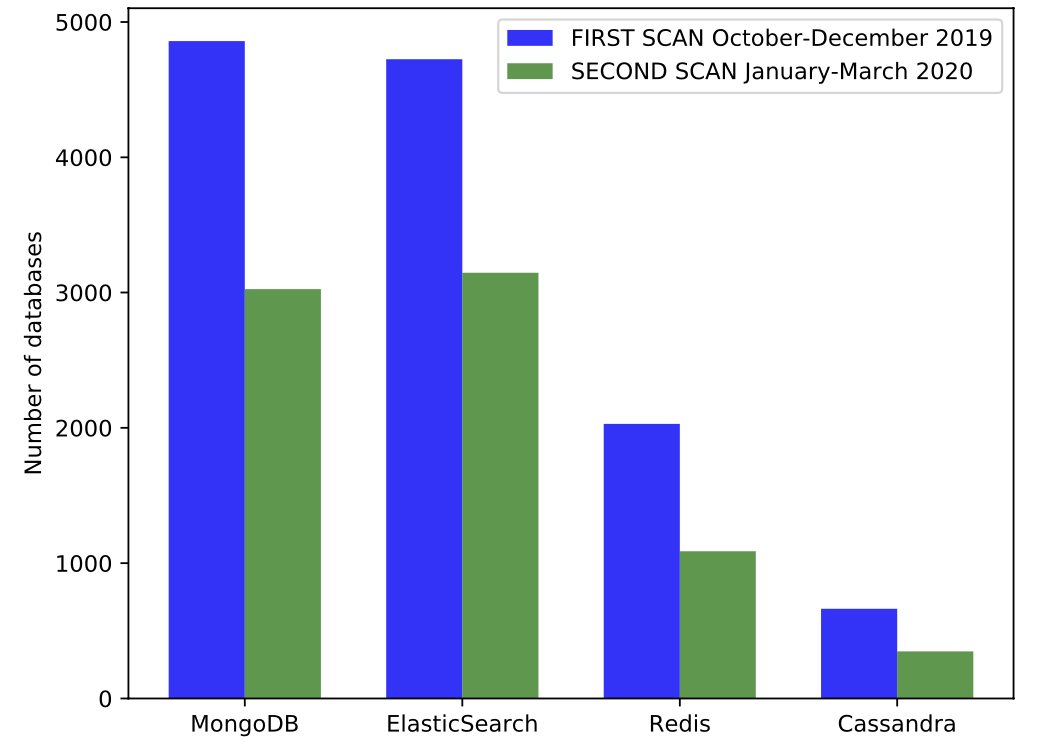
\includegraphics[width=0.6\textwidth]{res/fig7.png}
    \caption{تاثیر آنالیز امنیتی: تعداد دیتابیس‌هایی که قبل و بعد از این آزمایش
    در خصوص پیکربندی نامناسب برسی شدند}
    \label{fig: diagram}
\end{figure}

\subsection{تجزیه و تحلیل نسخه سرویس‌های NoSQL}

خالی از لطف نیست که اشاره کنیم، محققان نسخه‌های استفاده شده از دیتابیس‌ها را نیز
مورد بررسی قرار دادند و متوجه شدند که تعداد زیادی از آنها از نسخه‌های قدیمی از
DBMS استفاده می‌کردند که دیگر توسط توسعه دهندگان ارائه دهندگان آنها دیگر
پشتیبانی نمی‌شد. به یاد داشته باشید که اگر از نسخه‌های قدیمی استفاده کنید ممکن
است آسیب پذیری را برای هکر‌ها آزاد کرده باشید که بتوانند از طریق آن به
دیتابیس‌ها و حتی اپلیکیشن‌های شما حمله کنند. مهم‌ترین هدف به روز رسانی‌ها دریافت
تمام پچ‌های امنیتی در سیستم‌های نرم‌افزار مخصوصا سیستم‌های خاص دیتابیسی است.
همچنین آگاه باشید که از چه نسخه‌ای از نرم‌افزار (در اینجا دیتابیس) استفاده
می‌کنید. نسخه مورد استفاده اگر در محیط Dev باشد آسیب پذیری بیشتری نسبت به
نرم‌افزار‌هایی دارند که در محیط Stable هستند. پس همیشه سعی کنید که از
نرم‌افزار‌های به روز Stable استفاده کنید.

\begin{figure}[H]
    \centering
    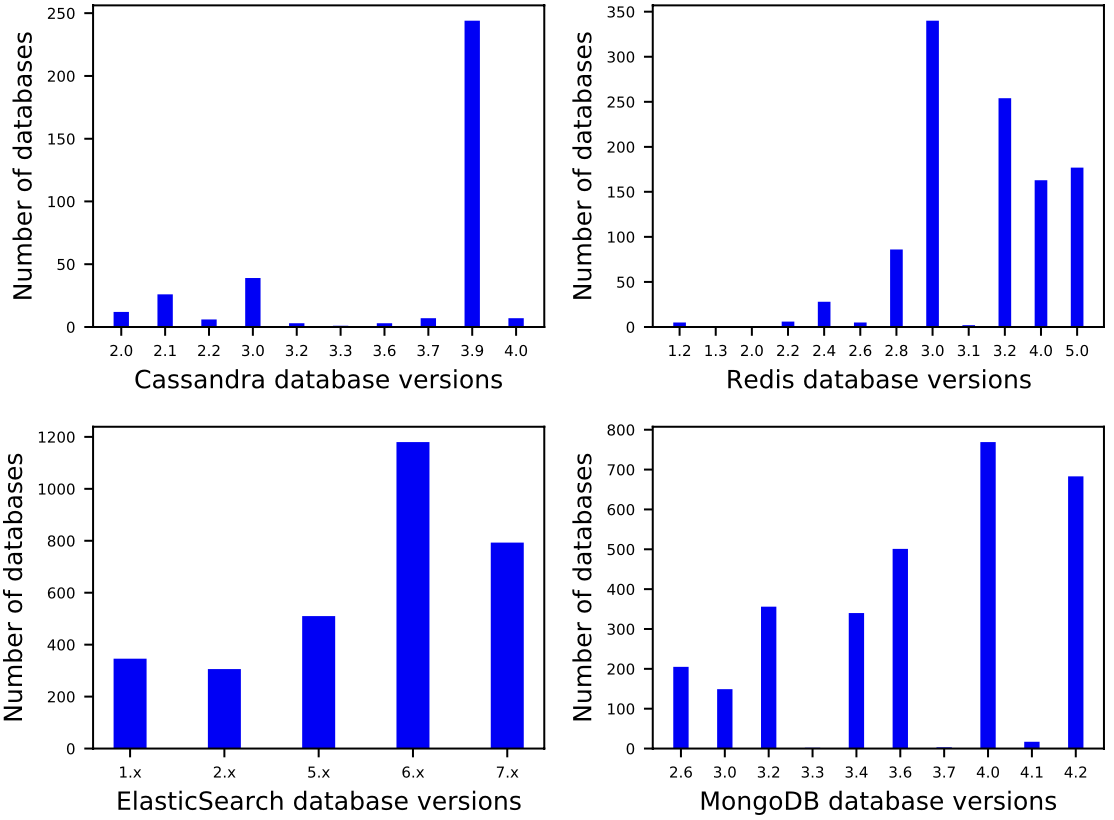
\includegraphics[width=0.6\textwidth]{res/fig8.png}
    \caption{بررسی نسخه سرویس‌های NoSQL}
    \label{fig: diagram}
\end{figure}

\section{جمع‌بندی}

در این گزارش در مورد محبوب‌ترین سرویس‌های دیتابییس NoSQL تحقیق کردیم. از طریق
ابزاری که محققان توسعه دادند پی‌بردیم که راه‌اندازی ساده و آسان درست است که کم
هزینست اما بعد از گذشت مدتی خیلی کم متوجه می‌شویم که هر چقدر برای راه‌اندازی
سیستم‌های دیتابیسی هزینه زمانی و مالی بگذاریم باز هم کم است. فریمورک محققان
براساس روندی امن این تحقیق را تسریع بخشید. فرایند‌های مختلفی در این بین بررسی
شدند. مانند حضور یک سیستم احرازهویت مناسب، عدم استقرار و راه‌اندازی سیستم‌های
داده‌ای در شماره پورت‌های پیش فرض و غیره. این بررسی برروی ۶۷ میلیون آدرس IP بین
اکتبر سال ۲۰۱۹ و مارس سال ۲۰۲۰ انجام شد. آسیب پذیری‌هایی که در حین خواندن این
گزارش شاهد بودید تنها ساده‌ترین آسیب پذیری‌هایی بودند که مورد بررسی قرار گرفتند.
همچنین انواع اهداف نفوذگران را بررسی کردیم که به چه شکلی می‌توانند تخریب اطلاعات
را انجام دهند. قلب تپنده یک سیستم اپلیکیشنی، کاربران و داده‌های آنها هستند. در
صورتی که داده‌ها فاش شود اعتماد به آن شبکه کم و به تدریج از بین می‌رود. این
تحقیق تنها روی ۴ دیتابیس مطرح شده صورت گرفت. به عنوان نمونه هنوز فرایندی که شاهد
آن بودید برروی دیتابیس‌های InfluxDB و دیگر دیتابیس‌های محبوب مانند Prometheus
انجام نشده است. همچنین محققان این مقاله به دنبال انجام این روند در بستر شبکه TCP
با استفاده از شناسایی آدرس‌های نسخه ۶ IP هستند.

\bibliographystyle{elsarticle-num}
\bibliography{lib.bib}

\end{document}